%
% Sección de estandares y recomendaciones del NIST
% Capítulo de análisis y diseño de generación de tokens.
% Proyecto Lovelace.
%

\subsection{Estándares y recomendaciones}

En esta sección se resumen los contenidos de los estándares y recomendaciones
del \gls{gl:nist} relacionados con los requerimientos planteados en la
sección anterior (\ref{sec:requerimientos}).

\begin{description}

  \item[Administración de llaves] (Sección \ref{sec:administracion_llaves})
    \begin{description}
      \item[800-57] \textit{Recommendation for Key Management}. Disponible en
        \cite{nist_llaves}.
      \item[800-130] \textit{A Framework for Designing Cryptographic Key
        Management Systems}. Disponible en \cite{nist_disenio_llaves}.
    \end{description}

  \item[Generación de llaves] (Sección \ref{sec:generacion_llaves})
    \begin{description}
      \item[800-108] \textit{Recommendation for Key Derivation Functions Using
        Pseudorandom Functions}. Disponible en \cite{nist_derivacion_llaves}.
      \item[800-133] \textit{Recommendation for Cryptographic Key Generation}.
        Disponible en \cite{nist_creacion_llaves}.
    \end{description}

  \item[Generación de bits pseudoaleatorios] (Sección
    \ref{sec:generadores_pseudoaleatorios})
    \begin{description}
      \item[800-90] \textit{Recommendation for Random Number Generation Using
        Deterministic Random Bit Generators}. Disponible en
        \cite{nist_aleatorios}.
    \end{description}
\end{description}

%
% Recomendaciones del NIST para la administración de llaves,
% capítulo de análisis y diseño para la generación de tokens.
% Proyecto Lovelace
%

\subsubsection{Administración de llaves}
\label{sec:administracion_llaves}

\paragraph{Tipos de llaves}

En \cite{nist_llaves}, el \gls{gl:nist} divide a las llaves criptográficas en
19 categorías, las cuales surgen de la combinación de la naturaleza de la
llave (simétrica, pública o privada) con la funcionalidad que se le da
(firmas, autenticación, cifrado, entre otras). En la tabla
\ref{clasificacion_llaves} se muestran dichas categorías: se marca con
$ \checkmark $ las combinaciones que tienen sentido práctico; por ejemplo, para
firmar (y posteriormente validar) solamente se ocupan las llaves de un esquema
asimétrico (i. e. públicas y privadas).

\begin{table}[H]
  \centering
  \begin{tabular}{| c | l | c | c | c |}

    \cline{3-5}
    \multicolumn{2}{c}{} &
    \multicolumn{3}{| c |}{\textbf{Naturaleza}} \\
    \cline{3-5}
    \multicolumn{2}{c |}{} &
    Simétrica &
    Pública &
    Privada \\
    \hline

    \multirow{10}{*}{\begin{sideways} \textbf{Funcionalidad} \end{sideways}}
    & Para firmas                        &            & \checkmark & \checkmark
    \\\cline{2-5}
    & Para autenticación                 & \checkmark & \checkmark & \checkmark
    \\\cline{2-5}
    & Para cifrado de datos              & \checkmark &            &
    \\\cline{2-5}
    & Como envoltura de otras llaves     & \checkmark &            &
    \\\cline{2-5}
    & Para generadores aleatorios        & \checkmark &            &
    \\\cline{2-5}
    & Como llave maestra                 & \checkmark &            &
    \\\cline{2-5}
    & Para el transporte de llaves       &            & \checkmark & \checkmark
    \\\cline{2-5}
    & Para el acuerdo de llaves          & \checkmark & \checkmark & \checkmark
    \\\cline{2-5}
    & Efímeras para el acuerdo de llaves &            & \checkmark & \checkmark
    \\\cline{2-5}
    & De autorización                    & \checkmark & \checkmark & \checkmark
    \\\hline

  \end{tabular}
  \caption{Clasificación de llaves criptográficas}
  \label{clasificacion_llaves}
\end{table}

\begin{description}

  \item[Para firmas:] llaves que son usadas en algoritmos asimétricos para
    generar firmas digitales con posibles implicaciones a largo plazo. Cuando
    son manejadas correctamente, este tipo de llaves está diseñado para
    proveer \gls{gl:autenticacion_origen}, autenticación de integridad y
    soporte para el no repudio.

  \item[Para autenticación:] son usadas para proporcionar garantías sobre la
    identidad de un fuente generadora (i. e. \gls{gl:autenticacion_origen}).

  \item[Para cifrado de datos:] usadas en esquemas simétricos para proveer de
    confidencialidad a la información (esto es, para cifrar la información).
    Como se tratan de algoritmos simétricos (o de llave secreta), la misma
    llave se usa para quitar la confidencialidad (para descifrar).

  \item[Como envoltura de otras llaves:] también llamadas llaves cifradoras de
    llaves (\textit{key-encrypting keys}), son usadas para proteger otras
    llaves usando algoritmos simétricos. Dependiendo del algoritmo con el que
    se use la llave, esta también puede ser usada para proveer de validaciones
    de integridad.

  \item[Para generadores aleatorios:] llaves usadas para generar números o bits
    aleatorios.

  \item[Como llaves maestra:] una llave maestra simétrica se usa para derivar
    otras llaves simétricas (p. ej. llaves de cifrado, o de envoltura). También
    se conoce como llave de derivación de llaves (\textit{key-derivation key}).

  \item[Para el transporte de llaves:] llaves utilizadas en esquemas
    asimétricos para proteger la comunicación en un proceso de acuerdo de
    llaves. Se usan para proteger otras llaves (p. ej. de cifrado, de
    envoltura) o información relacionada (p. ej.
    \glspl{gl:vector_de_inicializacion}).

  \item[Para el acuerdo de llaves:] utilizadas en algoritmos de acuerdo de
    llaves para establecer otras llaves. Generalmente funcionan en plazos muy
    largos.

  \item[Efímeras para el acuerdo de llaves:] llaves de muy corto plazo que son
    usadas una sola vez en un proceso de establecimiento de otras llaves. En
    algunos casos la llave efímera puede ser usada más de una vez, pero dentro
    de la misma transacción.

  \item[De autorización:] usadas para proveer y verificar los privilegios de
    una entidad. En un esquema simétrico, la llave es conocida tanto por la
    entidad que provee acceso, como por la que desea acceder.

\end{description}

%Además de las llaves, existen algunos otros parámetros que comunmente se usan
%en los algoritmos criptográficos, y que también necesitan ser tomados en
%consideración:
%
%\begin{description}
%
%  \item[Parámetros de dominio:] Son usados junto con algunos algoritmos de
%    llave pública para generar pares de llaves o crear firmas digitales.
%
%  \item[\glspl{gl:vector_de_inicializacion}:] usados en algunos
%    \glspl{gl:modo_de_operacion} (ver el glosario).
%
%  \item[Secretos compartidos:] son generados durante el proceso de acuerdo de
%    llaves. Estos deben ser manejados y protegidos de la misma forma que las
%    llaves criptográficas.
%
%  \item[Semillas de \gls{gl:rng}:] son usadas en la generación de números
%    aleatorios determinísticos.
%
%  \item[Otros datos públicos:] información pública extra que es usada durante
%    el proceso de establecimiento de llaves (por ejemplo los \textit{nonce}).
%
%  \item[Otros datos privados:] información secreta usada en el proceso de
%    establecimeinto de llaves (por ejemplo una semilla de un \gls{gl:rng}).
%
%  \item[Resultados intermedios:] resultados intermedios de operaciones
%    criptográficas; estos deben ser protegidos, y no deben ser usados de una
%    manera distinta a la establecida por el algoritmo criptgráfico.
%
%  \item[Información de control de llaves:] información relacionada al material
%    de llaves (\textit{keying material}), por ejemplo, el identificador, un
%    propósito, un contador, etcétera; se debe de proteger para poder asegurar
%    que esta información puede ser usada correctamente. La información de
%    control de llaves se debe incluir en los metadatos de una llave.
%
%  \item[Números aleatorios:] los números creados por un \gls{gl:rng} se deben
%    de proteger cuando se retengan.
%
%  \item[Contraseñas:] las contraseñas son usadas para adquirir privilegios de
%    acceso, y pueden ser usadas como credenciales en mecanismos de
%    \gls{gl:autenticacion_origen}. Las contraseñas también se pueden usar para
%    derivar llaves criptográficas que son usadas para protejer y acceder
%    a contenido alamcenado.
%
%  \item[Información de auditoría:] la infromación de auditorías contiene
%    registros de los eventos de la administración de llaves.
%
%\end{description}

\paragraph{Usos de llaves}

En general, las llaves se deben de utilizar para un solo propósito: el uso de
la misma llave para dos operaciones criptográficas puede debilitar la seguridad
provista por ambas; al limitar el uso de una llave se limita el nivel de riesgo
de que esta se vea comprometida; algunos usos de llaves interfieren unos
con otros.

La regla anterior no se extiende a situaciones en donde el mismo
proceso provea de múltiples servicios. Por ejemplo, cuando una sola firma
digital provee de autenticación de integridad y de autenticación de origen,
o cuando una sola llave simétrica es usada para cifrar y para autenticar en
una sola operación.

\paragraph{Criptoperiodos}

Un criptoperiodo es el rango de tiempo durante el cual una llave es válida.
Algunas de las funciones de los criptoperiodos son:

\begin{itemize}

  \item Limitar el total de daños si una sola llave se ve comprometida.

  \item Limitar el uso de un algoritmo en particular (\textit{particular}
    en el sentido de la instancia misma del algoritmo).

  \item Limitar el tiempo disponible para intentos de ataques sobre los
    mecanismos que protegen a la llave del acceso sin autorización.

  \item Limitar el periodo en el cual la información puede verse comprometida
    por revelaciones inadvertidas de llaves a entidades sin autorización.

  \item Limitar el tiempo disponible para ataque criptoanalíticos.

\end{itemize}

A continuación se enlistan los principales factores a tomar en cuenta al
momento de establecer un criptoperiodo:

\begin{itemize}

  \item La fuerza del mecanismo criptográfico (el algoritmo, la
    \gls{gl:fuerza_efectiva} de la llave, el tamaño de bloque, el modo de
    operación, etc.).

  % ¿La encarnación de los mecanismos?

  \item El entorno de operacion (p. ej. un lugar de acceso restringido, una
    terminal pública).

  \item El volumen de información transmitida, o el número de transacciones.

  \item La función de seguridad (cifrado de datos, firma digital, derivación
    de llaves, etc.).

  \item El método de entrada de la llave (por teclado, a nivel de sistema).

  \item El número de nodos en una red que comparten la misma llave.

  \item El número de copias de la llave distribuidas.

  \item Rotaciones de personal.

  \item La amenaza de los adversarios (¿de quién se está protegiendo la
    información?, ¿cuáles son sus capacidades?)

  \item La amenza de avances tecnológicos (nuevos límites para el problema
    del logaritmo discreto, computadoras cuánticas).

\end{itemize}

La duración de los criptoperiodos también debe tomar en cuenta cuáles son
los riesgos de las actualizaciones de llaves. En general, entre más cortos
sean los criptoperiodos, mejor; sin embargo, si los mecanismos de distribución
de llaves son manuales y propensos a errores humanos, entonces el riesgo se
invierte. En estos casos (en especial cuando se utiliza
\gls{gl:criptografia_fuerte}) resulta mejor tener pocas y bien controladas
distribuciones manuales, a que estas sean frecuentes y mal controladas.

Las consecuencias de una exposición se miden de acuerdo a qué tan sensible es
la información, qué tan críticos son los procesos protegidos, y qué tan alto
es el costo de recuperación en caso de exposición. La sensibilidad se refiere
al periodo de tiempo durante el cual la información debe estar protegida (5
segundos, 5 minutos, 5 horas o 5 años) y a las consecuencias potenciales en
caso de pérdida de protección. En general, entre más sensible sea la
información protegida, el criptoperiodo debe ser menor (sin llegar a que
sea contraproducente).

Algunos otros factores a tomar en cuenta incluyen el uso de las llaves y el
costo de actualizaciones. En cuanto al uso de las llaves, generalmente se
hace distinción en cuanto a si la información protegida solamente se está
transfiriendo, o si se va a almacenar; en general los criptoperiodos son más
largos en caso de almacenamiento, dado el costo que puede representar el
recifrado de toda una base de datos. Esto está relacionado con el costo de
las actualizaciones: cuando el volumen de información protegida es demasiado
grande o cuando esta se encuentra distribuida en distintos puntos geográficos,
el costo de un cambio de llaves puede ser demasiado elevado.

La tabla \ref{criptoperiodos_sugeridos} muestra las sugerencias del
\gls{gl:nist} en \cite{nist_llaves} en cuanto a la duración de los
criptoperiodos según cada tipo de llave.

\begin{table}[H]
  \centering
  \begin{tabular}{| p{0.5\textwidth} | p{0.2\textwidth} | p{0.2\textwidth} |}

    \hline
    \multirow{2}{*}{\textbf{Tipo de llave}} &
    \multicolumn{2}{ c |}{\textbf{Criptoperiodo}} \\
    \cline{2-3}
    & \textbf{Periodo de uso de emisor (PE)}
    & \textbf{Periodo de uso de receptor (PR)} \\
    \hline

    1.- Llave privada para firma &
    1 a 3 años &
    - \\
    \hline

    2.- Llave pública para verificación de firma &
    \multicolumn{2}{ c |}{Depende del tamaño de la llave} \\
    \hline

    3.- Llave simétrica para autenticación &
    $ \leq 2 $ años &
    $ \leq PE + 3 $ años \\
    \hline

    4.- Llave privada para autenticación &
    \multicolumn{2}{ c |}{1 a 2 años} \\
    \hline

    5.- Llave pública para autenticación &
    \multicolumn{2}{ c |}{1 a 2 años} \\
    \hline

    6.- Llave simétrica para cifrado de datos &
    $ \leq 2 $ años &
    $ \leq PE + 3 $ años \\
    \hline

    7.- Llave simétrica como envoltura &
    $ \leq 2 $ años &
    $ \leq PE + 3 $ años \\
    \hline

    8.- Llave simétrica para generadores aleatorios &
    ver SP800-90 &
    - \\
    \hline

    9.- Llave simétrica maestra &
    alrededor de 1 año &
    - \\
    \hline

    10.- Llave privada para transporte &
    \multicolumn{2}{ c |}{$ \leq 2 $ años} \\
    \hline

    11.- Llave pública para transporte &
    \multicolumn{2}{ c |}{1 a 2 años} \\
    \hline

    12.- Llave simétrica para acuerdo &
    \multicolumn{2}{ c |}{1 a 2 años} \\
    \hline

    13.- Llave privada para acuerdo &
    \multicolumn{2}{ c |}{1 a 2 años} \\
    \hline

    14.- Llave pública para acuerdo &
    \multicolumn{2}{ c |}{1 a 2 años} \\
    \hline

    15.- Llave privada efímera para acuerdo &
    \multicolumn{2}{ c |}{Solo 1 transacción} \\
    \hline

    16.- Llave pública efímera para acuerdo &
    \multicolumn{2}{ c |}{Solo 1 transacción} \\
    \hline

    17.- Llave simétrica para autorización &
    \multicolumn{2}{ c |}{$ \leq 2 $ años} \\
    \hline

    18.- Llave privada para autorización &
    \multicolumn{2}{ c |}{$ \leq 2 $ años} \\
    \hline

    19.- Llave pública para autorización &
    \multicolumn{2}{ c |}{$ \leq 2 $ años} \\
    \hline

  \end{tabular}
  \caption{Criptoperiodos sugeridos por tipo de llave}
  \label{criptoperiodos_sugeridos}
\end{table}

% Demasiado abstracto:
%
%\paragraph{Garantías}
%
%Cuando una llave es almacenada o distribuida, podría pasar por entornos
%inseguros; es por esto por lo que antes de usarse para sus operaciones
%criptográficas normales, una llave debe cumplir con las siguientes garantías.
%
%\begin{description}
%
%  \item[Garantía de integridad:] como mínimo, la integridad se debe obtener
%    verificando que el material de la llave tiene el formato correcto y
%    proviene de fuentes autorizadas. De manera adicional se pueden usar
%    códigos de detección de error, códigos de autenticación de mensaje y
%    firmas digitales.
%
%  \item[Garantía de validez de parámetros de dominio:] los parámetros de
%    dominio son usados por los algoritmos de llave pública al momento de la
%    generación de llaves y firmas digitales, y durante la generación de
%    secretos compartidos. Esta garantía es muy importante, y se debe obtener
%    antes de usar el algoritmo.
%
%  \item[Garantía de validez de llave pública:] esta validación permite al
%    usuario estar seguro de que la llave pública es aritméticamente correcta.
%    Esto reduce las posibilidades de usar llaves débiles o corruptas. Una de
%    varias maneras de obtener esta garantía es mediante la verificación de
%    algunas propiedades matemáticas que la llave pública debe tener (estas
%    dependen según el algoritmo).
%
%  \item[Garantía de posesión de llave privada:] esta garantía debe ser obtenida
%    por ambas partes: el dueño de los pares y las demás entidades que
%    reciben la llave pública. Los métodos para obtener la garantía son
%    específicos a cada algoritmo.
%
%\end{description}

\paragraph{Estados de llaves y transiciones}

En la figura \ref{estados_de_llaves} se muestra un diagrama de estados con
los posibles comportamientos de una llave criptográfica. Un criptoperiodo
inicia al entrar en el estado «activo» (transición 4) y termina al llegar al
estado «destruido». En el caso de esquemas asimétricos, las transiciones se
aplican a ambos pares de llaves. Se debe llevar un registro de la fecha y hora
(y en algunos casos de las razones) de cualquier cambio de estado.

\begin{figure}
  \begin{center}
    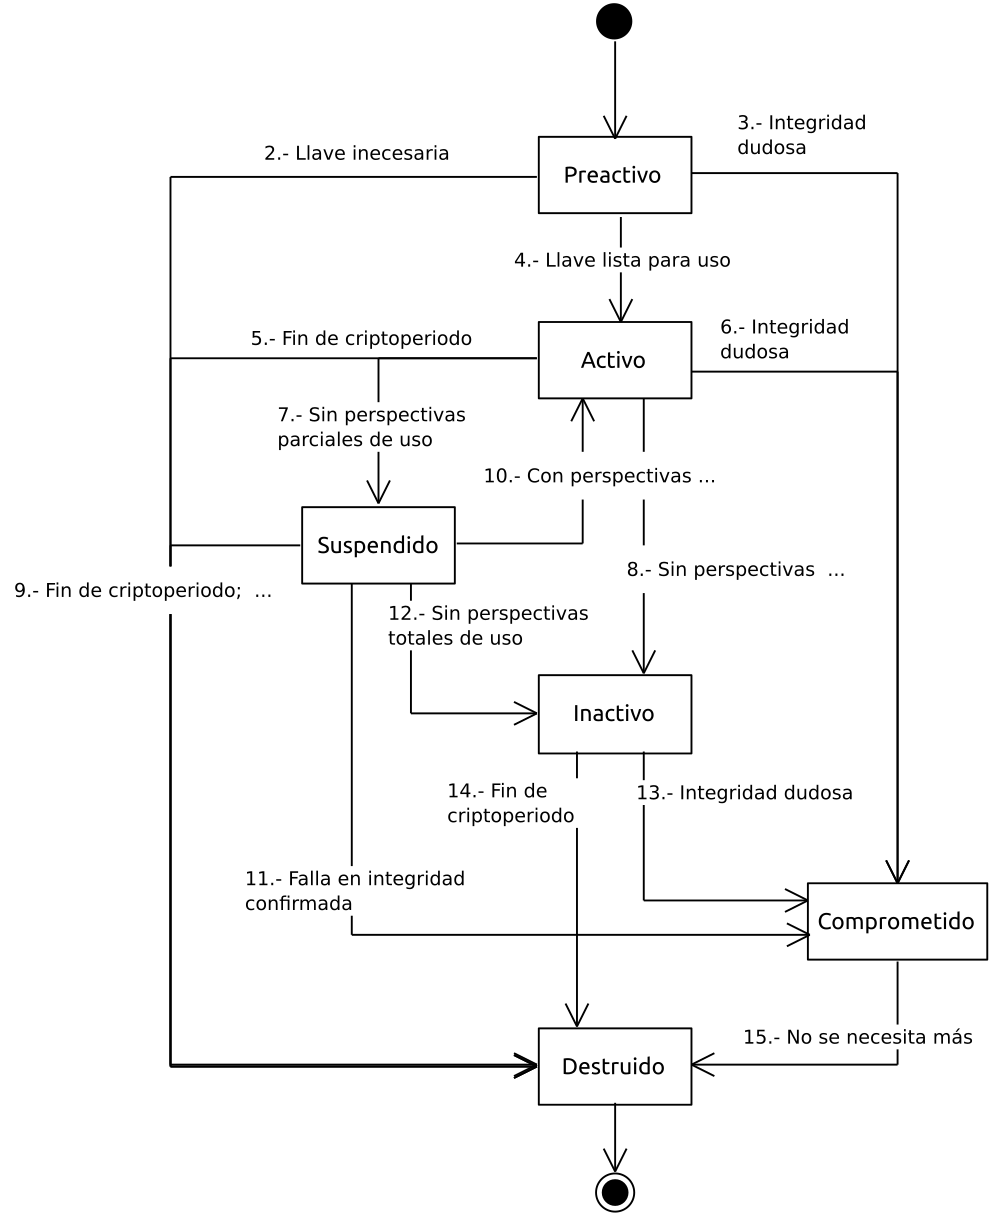
\includegraphics[width=0.8\linewidth]{diagramas/estados_de_llaves.png}
    \caption{Diagrama de estado de llaves criptográficas.}
    \label{estados_de_llaves}
  \end{center}
\end{figure}

Hay varias posibles razones por las que se puede llegar a un estado
«suspendido»: la entidad dueña de una firma digital no se encuentra disponible;
se sospecha que la integridad de la llave está comprometida, por lo que se pasa
a este estado en lo que se investiga más en profundidad; entre otros. Una
llave que está en este estado («suspendido») no debe ser usada bajo ninguna
circunstancia.

Las llaves que se encuentran en el estado «inactivo» no deben ser usadas para
aplicar protección criptográfica, pero en algunos casos, pueden ser usadas
para procesar información protegida con criptografía. Por ejemplo, las llaves
simétricas usadas para autenticación, cifrado de datos o envoltura de llaves,
pueden ser usadas para procesar información hasta que acabe el periodo del
emisor de la llave emisora.

El estado «comprometido» representa a las llaves a las que una entidad sin
autorización tiene o ha tenido acceso. Las llaves comprometidas no deben ser
usadas para aplicar protección criptográfica, sin embargo, en algunos casos
es posible que sean usadas para procesar información (en condiciones
sumamente controladas); por ejemplo, si la cierta información fue firmada
antes de que se produjera la brecha de seguridad, las llaves pueden ser
usadas para valida esta firma.

%
% Recomendaciones del NIST para la generación de llaves,
% capítulo de análisis y diseño para la generación de tokens.
% Proyecto Lovelace.
%

\subsubsection{Generación de llaves}
\label{sec:generacion_llaves}

% NIST 800-133 ---

\paragraph{Generación de llaves en general}

\subparagraph{Métodos para la generación de llaves}
La generación de llaves se puede hacer por medio del uso de generadores de
bits aleatorios (\gls{gl:rbg}), de la derivación de llaves a partir de otras,
de la derivación de llaves a partir de una contraseña, y del uso de un esquema
de acuerdo entre llaves o \textit{key agreement}; pero todas, de forma directa
o indirecta deben estar basadas en la salida de un \gls{gl:rbg}.

\subparagraph{Donde generar las llaves}
La generación de llaves criptográficas debe ir de acuerdo con el \gls{gl:fips}
140 (descrito en \cite{nist_modulos_criptograficos}), y si es necesario que
las llaves sean transferidas, se debe de hacer por medio de un canal seguro.
Además, todos los valores aleatorios requeridos para la generación de las
llaves deben ser generados dentro de un mismo módulo criptográfico.

\subparagraph{Fuerza de la seguridad}
La fuerza de la seguridad de un método es una medición de la complejidad
asociada a la recuperación de información secreta o de la seguridad relativa
a un algoritmo criptográfico a partir de datos conocidos.

Se dice que un método soporta la fuerza de seguridad, si la fuerza de
seguridad provista por dicho método es igual o mayor a la seguridad
requerida para la protección de la información.
\begin{itemize}

  \item La fuerza de seguridad para los \gls{gl:rbg} está basada en la
    \gls{gl:entropia} o aleatoriedad que provee el mismo \gls{gl:rbg}.

  \item La seguridad de un algoritmo criptográfico se basa en el hecho de
    que las llaves que usan fueron generadas por medio de procesos que las
    proveyeron de una \gls{gl:entropia} mayor o igual a la necesaria para el
    algoritmo, así como el mismo tamaño de las llaves.

  \item La fuerza de seguridad de una llave depende del algoritmo que la
    utilizará, su tamaño, el proceso con el que fue generada, y la forma en
    la que es utilizada.

\end{itemize}

\subparagraph{Usos de las salidas de los \gls{gl:rbg}}
Suponiendo que $K$ es una llave simétrica o un valor aleatorio que sirve
como entrada de un algoritmo generador de pares de llaves asimétricas, $K$
debe ser una cadena de bits tal que:
\begin{equation}
  \label{bits_K}
  K\: =\: U\: \oplus\: V
\end{equation}
donde $U$ es una cadena de bits que se obtuvo de un \gls{gl:rbg} con el
soporte de la fuerza de seguridad requerida, y $V$ es una cadena de bits de la
misma longitud, que además fue generada de manera tal que es independiente de
$U$ y viceversa. La independencia entre $U$ y $V$ se requiere debido a que se
tiene que evitar que el conocimiento de alguna de estas cadenas pueda usarse
para obtener información de la otra.

\subparagraph{Generación de pares de llaves asimétricas}
Los pares de llaves solo pueden ser generados o por el propietario del las
mismas llaves, o por un tercero de confianza capaz de proveerlas.

Las llaves privadas deben permanecer secretas dentro del módulo criptográfico
del propietario o de un tercero de confianza, además de que, si se tienen que
transferir dichas llaves, se debe de garantizar que solo el propietario o la
parte generadora puedan verlas en claro.

\subparagraph{Generación de llaves simétricas}
Las llaves deben de ser generadas por una o varias de las entidades que
las compartirán, o por un tercero de confianza capaz de compartirlas de una
manera segura.

Las llaves que son generadas directamente de un \gls{gl:rbg} deben de cumplir
con la forma establecida en la ecuación \ref{bits_K}.

Cuando sea necesario compartir una llave, su distribución debe de ser manual,
o por medio de un envolvimiento de la misma o \textit{key wrapping}, el cual
debe de soportar la fuerza de seguridad requerida para la protección de la
información que protege la llave.

Obtener llaves derivadas de una contraseña es una práctica cuestionable,
debido a que comúnmente la aleatoriedad en las contraseñas es mínima, por tal
razón al generarse llaves de esta manera, es fuertemente recomendado que los
usuarios seleccionen contraseñas con una gran cantidad de \gls{gl:entropia}.
De cualquier manera, se considera que este tipo de llaves proveen una
\gls{gl:entropia} nula, a menos que la contraseña haya sido generada con
un \gls{gl:rbg}.

Cuando se tiene un conjunto de llaves $K_1, \dots, K_n$ generadas de forma
independiente, estas pueden ser combinadas entre sí para formar una llave $K$.
Igualmente, si se tiene un conjunto de bloques de información $V_1, \dots,
V_m$ que son independientes de sus respectivas llaves, se pueden combinar
estos bloques y sus llaves para formar otra llave.

Los métodos aprobados para generar llaves a partir de la combinación de
otras son:
\begin{itemize}

  \item La concatenación de varias llaves.
    $K\: =\: K_1\: \parallel\: \dots\: \parallel\: K_n$.

  \item La aplicación de compuertas \textit{xor} (o exclusiva) a varias llaves.
    $K\: =\: K_1\: \oplus\: \dots\: \oplus\: K_n$.

  \item La aplicación de compuertas \textit{xor} (o exclusiva) a varias llaves
    y bloques de información.
    $K\: =\: K_1\: \oplus\: \dots\: \oplus\: K_n\:
    \oplus\: V_1\: \oplus\: \dots\: \oplus\: V_m$.

\end{itemize}

Cuando sea necesario reemplazar una llave, la nueva llave debe de ser
completamente independiente de la anterior, para que el conocimiento de esta
última, no proporcione ningún conocimiento de la nueva.

% NIST 800-108 ---

\paragraph{Funciones Pseudoaleatorias (PRF)}

Las funciones pseudoaleatorias o \gls{gl:prf} (ver sección
\ref{sec:generadores_pseudoaleatorios}) son funciones computables en
\gls{gl:tiempo_polinomial} con un índice o \gls{gl:semilla} $s$ y una variable
de entrada $x$, de manera que cuando $s$ se selecciona aleatoriamente de $S$,
es \gls{gl:computacionalmente_indistinguible} de una función aleatoria
definida en el mismo dominio y rango que $PRF(s,x)$.

Cuando una llave criptográfica $K_I$ es usada como la \gls{gl:semilla} de una
\gls{gl:prf}, su salida se puede utilizar como \gls{gl:material_de_llaves}.

Para la derivación de llaves se tiene permitido el uso del \gls{gl:hmac} o
del \gls{gl:cmac} como función pseudoaleatoria.

\paragraph{Funciones de derivación de llaves (KDF)}

Las funciones de derivación de llaves o \gls{gl:kdf} son funciones que a
partir de una llave dada como entrada, pueden generar
\gls{gl:material_de_llaves} capaz de ser empleado por varios algoritmos
criptográficos.

Las llaves de entrada de este tipo de funciones son llamadas \textit{key
derivation keys} y deben ser llaves criptográficas generadas por medio de un
\gls{gl:rbg} o por un proceso automático de establecimiento de llaves.

El \gls{gl:material_de_llaves} segmentado es usado como un conjunto de llaves
criptográficas correspondientes a distintos algoritmos que pueden ofrecer
diferentes servicios, por lo tanto las \gls{gl:kdf} deben de definir una
manera de transformar este material en llaves distintas.

De forma general las \gls{gl:kdf} funcionan iterando $n$ veces una función
pseudoaleatoria para concatenar sus salidas hasta que se alcance la longitud
de bits deseada para el \gls{gl:material_de_llaves}.

\paragraph{Modos de iteración}

Algo necesario para el funcionamiento de las \gls{gl:kdf} son los modos de
iteración, ya que definen las entradas que se tendrán y el orden de los campos
de salida en cada ciclo.

\subparagraph{Counter mode}
En la figura \ref{diagrama_counter_mode} se aprecia la forma de operación de
este modo de iteración, en el que los datos de entrada son concatenados en una
cadena binaria de la forma: $Label \parallel 0x00 \parallel Context \parallel
{[L]}_2$ donde el $Label$ es un valor que identifica el propósito del
\gls{gl:material_de_llaves}, $0x00$ es un octeto de ceros, el $Context$ es una
cadena con la información relacionada al \gls{gl:material_de_llaves}, y
${[L]}_2$ es la longitud del \gls{gl:material_de_llaves} que se desea obtener
representada en binario. Como se observa, en este modo de iteración el
contador forma parte los datos de entrada de la \gls{gl:prf}.

\begin{figure}
  \begin{center}
    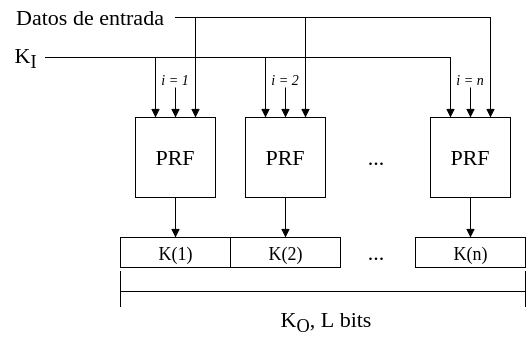
\includegraphics[width=0.75\linewidth]{diagramas/counter_mode}
    \caption{Diagrama del \textit{counter mode}.}
    \label{diagrama_counter_mode}
   \end{center}
\end{figure}

%Pseudocodigo excediéndose de los 80 para una correcta visualización el en pdf
\begin{pseudocodigo}[caption={Funcionamiento del \textit{counter mode}.},
label={mi:1}]
    entrada:   La llave $K_I$, la longitud $L$ y los valores de $Label$ y $Context$.
    salida:    $K_O$, con una longitud de $L$ bits.
    inicio
      calcular $n\: =\: [\frac{L}{h}]$, donde $h$ es la longitud de salida de la $PRF$.
      si $n$ > $2^r-1$, indicar error y parar; donde $r\: \leq\: 32$.
      $resultado(0) = \emptyset$
      para $i=1$ hasta $n$:
        $K(i)\: =\: PRF(K_I,\: {[i]}_2 \parallel Label \parallel 0x00 \parallel Context \parallel {[L]}_2 )$.
        $resultado(i)\: =\: resultado(i-1) \parallel K(i)$.
      $K_O =$ los L bits más a la izquierda del $resultado(n)$.
    fin
\end{pseudocodigo}

\subparagraph{Feedback mode}
Este modo de iteración opera tomando la salida de la \gls{gl:prf} en la
iteración anterior como parte los datos de entrada de la iteración actual.
Cabe resaltar que como se muestra en la figura \ref{diagrama_feedback_mode},
es opcional tener un contador concatenado a estos datos, que son iguales que
en el modo de operación anterior, solo que con un
\gls{gl:vector_de_inicializacion} $IV$.

\begin{figure}
  \begin{center}
    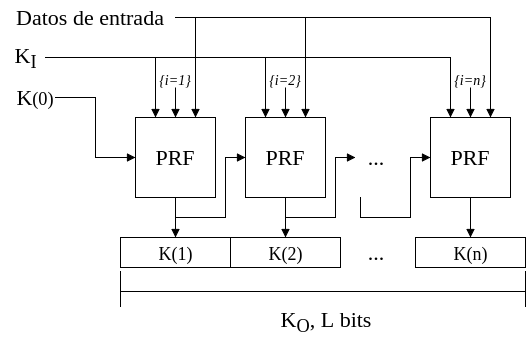
\includegraphics[width=0.75\linewidth]{diagramas/feedback_mode}
    \caption{Diagrama del \textit{feedback mode}.}
    \label{diagrama_feedback_mode}
   \end{center}
\end{figure}

%Pseudocodigo excediéndose de los 80 para una correcta visualización el en pdf
\begin{pseudocodigo}[caption={Funcionamiento del \textit{feedback mode}.},
label={mi:2}]
    entrada:   La llave $K_I$, la longitud $L$, el vector de inicialización IV
               y los valores de $Label$ y $Context$.
    salida:    $K_O$, con una longitud de $L$ bits.
    inicio
      calcular $n\: =\: [\frac{L}{h}]$, donde $h$ es la longitud de salida de la $PRF$.
      si $n$ > $2^{32}-1$, indicar error y parar.
      $resultado(0)\: =\: \emptyset$.
      $K(0) = IV$.
      para $i=1$ hasta $n$:
        $K(i)\: = \:PRF(K_I,\: K(i-1)\: \{\parallel {[i]}_2\}\: \parallel Label \parallel 0x00 \parallel Context \parallel {[L]}_2 )$.
        $resultado(i)\: =\: resultado(i-1) \parallel K(i)$.
      $K_O =$ los L bits más a la izquierda del $resultado(n)$.
    fin
\end{pseudocodigo}

\subparagraph{Double pipeline mode}
Como su nombre lo indica y a diferencia de los otros dos modos de iteración
mencionados, este usa dos flujos, donde un flujo es el encargado de generar
valores secretos, y el otro usa como entradas las salidas del primero para
obtener $K_O$. Los datos de entrada son iguales que en el primer modo de
iteración mencionado, y su funcionamiento está descrito en la figura
\ref{diagrama_dpipeline_mode}.

\begin{figure}
  \begin{center}
    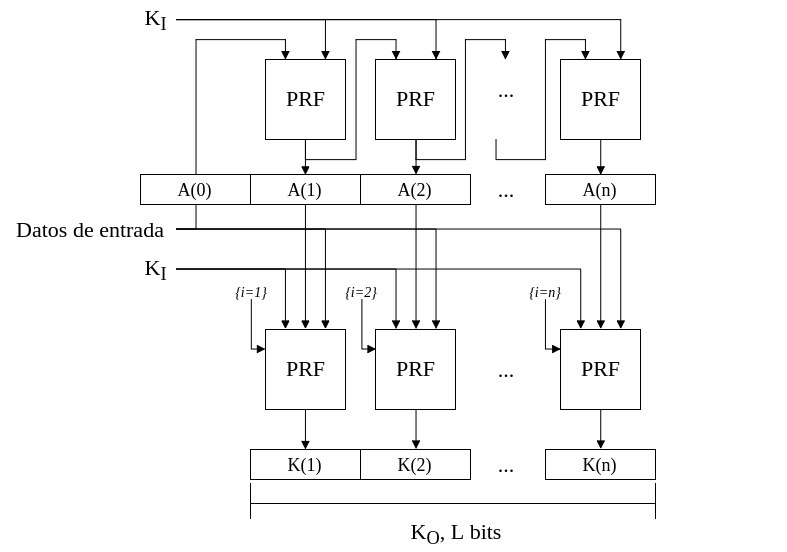
\includegraphics[width=0.75\linewidth]{diagramas/dpipeline_mode}
    \caption{Diagrama del \textit{double pipeline mode}.}
    \label{diagrama_dpipeline_mode}
   \end{center}
\end{figure}

%Pseudocodigo excediéndose de los 80 para una correcta visualización el en pdf
\begin{pseudocodigo}[caption={Funcionamiento del \textit{double pipeline mode}.},
label={mi:3}]
    entrada:   La llave $K_I$, la longitud $L$ y los valores de $Label$ y $Context$.
    salida:    $K_O$, con una longitud de $L$ bits.
    inicio
      calcular $n\: =\: [\frac{L}{h}]$, donde $h$ es la longitud de salida de la PRF.
      si $n$ > $2^{32}-1$, indicar error y parar.
      $resultado(0)\: =\: \emptyset$.
      $A(0)\: =\: IV\: =\: Label \parallel 0x00 \parallel Context \parallel {[L]}_2$
      para $i=1$ hasta $n$:
        $A(i)\: =\: PRF(K_I, A(i-1))$.
        $K(i)\: =\: PRF(K_I,\: A(i)\: \{\parallel {[i]}_2\}\: \parallel Label \parallel 0x00 \parallel Context \parallel {[L]}_2)$.
        $resultado(i) = resultado(i-1) \parallel K(i)$.
      $K_O =$ los L bits más a la izquierda del $resultado(n)$.
    fin
\end{pseudocodigo}

\subparagraph{Jerarquía de llaves}
El \gls{gl:material_de_llaves} proveniente de una derivación puede ser usado
una o más veces como llave de entrada de otras derivaciones subsecuentes, así,
es posible establecer una jerarquía en la que las llaves tienen distintos
niveles.

\paragraph{Consideraciones de seguridad}

\subparagraph{Fuerza criptográfica}
La fuerza de seguridad de una \gls{gl:kdf} es medida por la cantidad de
trabajo requerido para distinguir su cadena de salida de una cadena de bits
que en verdad tenga una \gls{gl:distribucion_uniforme} y cuente con la misma
longitud, suponiendo que la llave de entrada $K_I$, es la única entrada
desconocida para la \gls{gl:kdf}.

\subparagraph{La longitud de la llave de entrada}
En algunas \gls{gl:kdf} el tamaño de la llave $K_I$ está definido por la
\gls{gl:prf} que usan internamente, por ejemplo cuando se usa el \gls{gl:cmac},
pero igualmente, otras \gls{gl:kdf} pueden usar llaves de cualquier tamaño,
como al usar el \gls{gl:hmac} como \gls{gl:prf}.

\subparagraph{Transformación de material de llaves a llaves criptográficas.}
La longitud en bits del \gls{gl:material_de_llaves} está limitada tanto por
el algoritmo relacionado a la salida de la \gls{gl:kdf}, como por el modo de
iteración que se usa.

\subparagraph{Codificación de los datos de entrada}
La información de entrada de una \gls{gl:kdf} consiste en diferentes campos
de datos, estos deben de estar ordenados de forma específica y sin ambigüedad,
de manera que se tenga un método de codificación capaz de mapear cada campo
individualmente. Esto es necesario para poder detectar ataques a la
\gls{gl:kdf} que dependan de la manipulación de esta información.

\subparagraph{Separación entre llaves}
Las llaves provenientes del \gls{gl:material_de_llaves} deben de estar
separadas criptográficamente, de tal manera que no se comprometa la seguridad
de ninguna de estas llaves derivadas. Cuando el \gls{gl:material_de_llaves}
se obtiene de múltiples ejecuciones de la \gls{gl:kdf} usando la misma llave
de entrada $K_I$, la \gls{gl:kdf} debe de garantizar que el
\gls{gl:material_de_llaves} de una ejecución no comprometa al de cualquier
otra.

\subparagraph{Enlace de contexto}
Todo el \gls{gl:material_de_llaves} debe estar ligado a todas las entidades
relacionadas para poder evitar errores de protocolo.

%
% Recomendaciones del NIST para la generación de bits pseudoaleatorios,
% capítulo de análisis y diseño para la generación de tokens.
% Proyecto Lovelace.
%

\subsubsection{Generación de bits pseudoaleatorios}
\label{sec:generadores_pseudoaleatorios}

Existen dos maneras de generar bits aleatorios: la primera es producir bits
de manera no determinística, donde el estado de cada uno (uno o cero) está
determinado por un proceso físico impredecible. Estos generadores de bits
aleatorios (\gls{gl:rbg}) son conocidos como generadores no determinísticos, o
\gls{gl:nrbg}. La otra manera, que será explorada a continuación, es calcular
determinísticamente los bits mediante un algoritmo; estos generadores
determinísticos son conocidos como \gls{gl:drbg}.

Un \gls{gl:drbg} tiene un mecanismo que utiliza un algoritmo que produce una
secuencia de bits partiendo de un valor inicial que es determinado por una
\gls{gl:semilla} que, a su vez, está determinada por la salida de la fuente de
aleatoriedad. Una vez que se tiene la \gls{gl:semilla} y se determina el valor
inicial, el \gls{gl:drbg} es instanciado y puede producir valores. Dado a su
naturaleza determinística, se dice que los valores producidos por el
\gls{gl:drbg} son pseudoaleatorios y no aleatorios; si la \gls{gl:semilla} es
mantenida oculta y el algoritmo fue bien diseñado, los bits de salida del
\gls{gl:drbg} serán impredecibles.

Un \gls{gl:drbg} debe implementar un mecanismo aprobado por el SP800-90A y, al
menos una fuente de aleatoriedad aprobada; además, puede incluir fuentes
complementarias, tales como fuentes para \glspl{gl:nonce}, cadenas de
personalización y entradas adicionales.

%% MODELO DE UN DRBG

La entrada de \gls{gl:entropia} es provista a un mecanismo \gls{gl:drbg} para
obtener una \gls{gl:semilla} utillizando una fuente de aleatoriedad. La entrada
de \gls{gl:entropia} y la \gls{gl:semilla} deben mantenerse secretas; que estos
valores permanezcan secretos es una de las bases de la seguridad del
\gls{gl:drbg}. Otras entradas, como un \gls{gl:nonce} o una cadena de
personalización pueden ser utilizadas como entradas; estas pueden o no requerir
ser mantenidas secretas también, y ser utilizadas para crear la \gls{gl:semilla}
inicial para el \gls{gl:drbg}.

El estado interno es la memoria del \gls{gl:drbg} y consiste en todos los
valores que requiere el mecanismo (parámetros, variables, etcétera).

El mecanismo \gls{gl:drbg} requiere cinco funciones; estas son explicadas con
más detalle abajo:
\begin{enumerate}
    \item Instanciación (\textit{instantiate function}): obtiene la entrada de
        \gls{gl:entropia} para crear una \gls{gl:semilla} con la cual será
        creado un nuevo estado interno. La entrada puede ser combinada con
        una \gls{gl:nonce} o una cadena de personalización.
    \item Generación (\textit{generate function}): genera bits pseudoaleatorios
        utilizando el estado interno actual; también tiene como salida un nuevo
        estado interno que es utilizado para el siguiente pedido.
    \item Cambio de \gls{gl:semilla} (\textit{reseed function}): obtiene una
        nueva entrada de \gls{gl:entropia} y la combina con el estado interno
        actual para crear una nueva \gls{gl:semilla} y un nuevo estado interno.
    \item Desinstanciación (\textit{uninstantiate function}): elimina el estado
        interno actual.
    \item Prueba de salud (\textit{healt htest function}): determina que el
        mecanismo \gls{gl:drbg} siga funcionando correctamente.
\end{enumerate}

Cuando a un \gls{gl:drbg} se le aplica la función de cambio de \gls{gl:semilla},
la \gls{gl:semilla} es imperativo que la \gls{gl:semilla} sea distinta a la que
se utilizó en la función de instanciación. Cada \gls{gl:semilla} define un nuevo
periodo de \gls{gl:semilla} (\textit{seed period}) para la instanciación del
\gls{gl:drbg}. Una instanciación consiste en uno o más periodos de
\gls{gl:semilla}, estos comienzan cuando se obtiene una nueva \gls{gl:semilla} y
terminan cuando la siguiente \gls{gl:semilla} es obtenida o el \gls{gl:drbg}
deja de utilizarse.

El estado interno deriva de la \gls{gl:semilla}; este incluye el estado de
trabajo (uno o más valores derivados de la \gls{gl:semilla} que deben
permanecer secretos, y la cuenta con el número de salidas que se han producido
con esa semilla) y la información administrativa (el nivel de seguridad, etc).
Es menester proteger el estado interno del \gls{gl:drbg}. La implementación del
mecanismo \gls{gl:drbg} puede haber sido diseñado para tener múltiples
instancias; en este caso, cada instancia debe tener su propio estado interno y
el estado interno de una instancia \gls{gl:drbg} jamás debe ser utilizado como
estado interno para una instancia distinta. El estado interno no debe ser
accesible a funciones distintas a las cinco del \gls{gl:drbg}, ni a otras
instancias del \gls{gl:drbg} o a otros \gls{gl:drbg}.

Los mecanismos especificados en \cite{nist_aleatorios} soportan cuatro niveles
de seguridad: 112, 128, 192 y 256 bits. Este es uno de los parámetros que
se necesitan para instanciar un \gls{gl:drbg}; además, dependiendo de su diseño,
cada mecanismo  \gls{gl:drbg} tiene sus restricciones de nivel de seguridad.
El nivel de seguridad depende de la implementación del \gls{gl:drbg} y la
cantidad de \gls{gl:entropia} que se da como entrada a la función de
instanciación.

Los bits pseudoaleatorios obtenidos mediante un \gls{gl:drbg} no deben ser
utilizados por una aplicación que requiera un nivel mayor de segurdad que con el
que fue instanciado el \gls{gl:drbg}. La concatenación de dos salidas del
\gls{gl:drbg} tampoco proveen un nivel de seguridad más alto que del que fueron
instanciados (por ejemplo, dos cadenas concatenadas de 128 bits no dan como
resultado una cadena de 256 bits con el nivel de seguridad de 256 bits).

\paragraph{\Glspl{gl:semilla}}

\paragraph{Funciones}

\paragraph{Mecanismos basados en funciones hash}

\paragraph{Mecanismos basados en cifradores por bloque}

\paragraph{Funciones auxiliares}

\paragraph{Garantías}

\paragraph{Documentación mínima}

\paragraph{Pruebas}

\paragraph{Errores}

